% Elipsoide del tensor: semiejes = ejes principales (autovectores)
\documentclass[border=5pt]{standalone}
\usepackage{tikz}
\usetikzlibrary{arrows.meta, calc}
\begin{document}
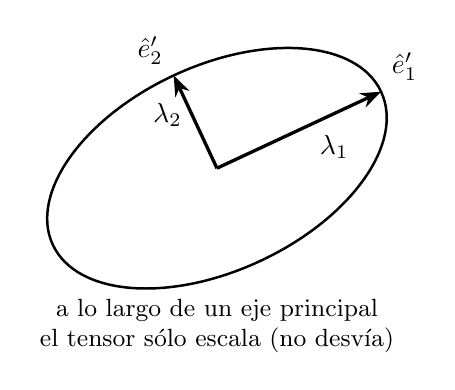
\begin{tikzpicture}[>={Stealth[length=2.6mm]}, line width=0.7pt]
  \coordinate (O) at (0,0);
  % elipse (corte del elipsoide) inclinada 25°
  \draw[rotate=25, line width=0.9pt] (0,0) ellipse (2.3 and 1.3);
  % ejes principales (autovectores)
  \draw[->, line width=1.2pt] (O)--(25:2.3) node[above right]{$\hat e'_1$};
  \draw[->, line width=1.2pt] (O)--(115:1.3) node[above left]{$\hat e'_2$};
  \node at (25:1.3) [below right] {$\lambda_1$};
  \node at (115:0.75) [left] {$\lambda_2$};
  % un vector aplicado a lo largo de e'_1 sólo se escala
  \node[align=center, font=\small] at (0,-2.0)
    {a lo largo de un eje principal\\ el tensor sólo escala (no desvía)};
\end{tikzpicture}
\end{document}
